% Compile with XeLaTeX twice from this directory.
\documentclass[10pt,a4paper]{article}
\usepackage{fontspec,unicode-math}
\setmainfont{TeX Gyre Termes}
\setsansfont{TeX Gyre Heros}[Scale=MatchLowercase]
\setmonofont{Latin Modern Mono}[Scale=0.82]
\setmathfont{STIX Two Math}
\usepackage[margin=22mm,headheight=14pt]{geometry}
\usepackage{microtype,booktabs,graphicx,amsmath,xcolor,hyperref,fancyhdr,enumitem}
\usepackage{xurl}
\usepackage{tikz}
\usepackage{pgfplots}
\pgfplotsset{compat=1.18}
\usetikzlibrary{arrows.meta,positioning}
\definecolor{accent}{HTML}{175A63}
\definecolor{cachelight}{HTML}{9BBBC0}
\definecolor{outputgold}{HTML}{BA8744}
\hypersetup{colorlinks=true,urlcolor=accent,linkcolor=accent,citecolor=accent,
  pdftitle={HCCA for Token-Efficient Repository Repair},pdfauthor={HCCA Project}}
\setlength{\parskip}{3pt}
\setlength{\parindent}{1em}
\setlist{nosep,leftmargin=*}
\pagestyle{fancy}
\fancyhf{}
\fancyhead[L]{\small\sffamily HCCA for Token-Efficient Repository Repair}
\fancyhead[R]{\small\sffamily Technical report}
\fancyfoot[C]{\small\thepage}
\renewcommand{\headrulewidth}{0.3pt}
% Derived from the versioned public summary.
\newcommand{\HRequests}{1,301}
\newcommand{\HInput}{36,810,516}
\newcommand{\HCached}{35,849,984}
\newcommand{\HMiss}{960,532}
\newcommand{\HOutput}{654,304}
\newcommand{\HReasoning}{408,903}
\newcommand{\HOtherOutput}{245,401}
\newcommand{\HCachePct}{97.3906}
\newcommand{\HInputM}{36.811}
\newcommand{\HOutputM}{0.654}
\newcommand{\HCost}{0.644212152}
\newcommand{\HCostPerResolved}{0.017895}
\newcommand{\BRequests}{2,014}
\newcommand{\BInput}{106,265,446}
\newcommand{\BCached}{104,137,856}
\newcommand{\BMiss}{2,127,590}
\newcommand{\BOutput}{4,050,837}
\newcommand{\BReasoning}{3,690,753}
\newcommand{\BOtherOutput}{360,084}
\newcommand{\BCachePct}{97.9979}
\newcommand{\BInputM}{106.265}
\newcommand{\BOutputM}{4.051}
\newcommand{\BCost}{3.062054268}
\newcommand{\BCostPerResolved}{0.087487}
\newcommand{\PairedSentence}{Both systems resolve 33 tasks, HCCA alone resolves 3, DSH alone resolves 2, and neither resolves 12.}

\title{\textbf{HCCA for Token-Efficient\\Repository Repair}}
\author{HCCA Project\\\small\url{https://github.com/klarisaka/HCCA-Official}}
\date{November 12, 2026}

\begin{document}
\maketitle
\thispagestyle{plain}

\begin{abstract}
Repeated code inspection, test output, and execution recovery can make the input
history of a coding agent expensive. HCCA assigns reading and execution work to
independent worker contexts backed by shared role prompts, with planning and
integration handled by a parent agent. We report a frozen direct-executor
configuration on all 50 tasks in a community-selected SWE-bench Verified Mini
dataset. HCCA v7 with low reasoning effort resolves 36 tasks, while a reused
DeepSeek Harness minimal high-effort baseline resolves 35. One HCCA task is
unfinished and receives zero credit in
the 50-task denominator. HCCA uses \HRequests{} model requests,
\HInputM{} million input tokens and \HOutputM{} million output tokens, with
\HCachePct{}\% of input reported as cached. At common off-peak token prices,
its normalized cost is \$\HCost{}, compared with a baseline known-complete
cost of at least \$\BCost{}. Both runs use the GXWTF endpoint, the
\texttt{deepseek-v4.1-flash} model alias and two concurrent tasks. HCCA's role
policy configures thinking/planning and analysts at high effort and
execution/reading at low. This direct-executor run records 1,301 low and zero
high requests. The baseline uses high. The observations support
an economical configuration on this manifest. They leave the separate
contributions of context design, prompts, tools and reasoning effort unresolved.
\end{abstract}

\section{Introduction}

Repository repair requires a coding agent to connect an issue description to
source code, make a change and test the resulting behavior. Each stage produces
material that may enter later model requests. A failed command can add a second
command, an explanation, and another output block. If every later request
contains this history, input consumption grows even when the final patch is
small. Provider-side prompt caching can reduce the price of repeated input,
while the total token volume and cache-miss volume remain important accounting
quantities.

HCCA organizes this work around reusable reader, executor and analyst roles.
A parent selects a bounded assignment and receives a compact result with
evidence references. The worker retains the detailed interaction needed for its
assignment. Shared role instructions provide a stable initial prompt segment,
and task details enter the subsequent conversation. This design is intended to
reduce the amount of execution history that must return to a planning context.

The present experiment concerns the direct-executor path through that runtime.
The local Root dispatcher invokes a low-effort executor immediately for each
repository issue, using the frozen configuration described in Section~3.

We examine task resolution, complete token accounting, cache reuse, output
composition and normalized monetary cost. We compare HCCA v7 with an already
completed minimal DeepSeek Harness (DSH) run on the same 50-task manifest.
Both systems use the same provider and model alias, with separate run dates and
different reasoning-effort settings. We retain the unfinished task in all
aggregate denominators and include its consumed tokens in cost.

\section{Runtime design}

\subsection{Shared roles and independent task contexts}

HCCA stores reusable reader and executor role configurations in a global agent
configuration directory. A newly delegated task receives the role instructions
and an assignment envelope. The worker then accumulates its own assistant and
tool messages. These role configurations can be reused across projects, while
each assignment starts a fresh conversation.

Readers inspect source and other necessary files. Executors inspect code,
modify the workspace, run commands and adapt to observed failures. Analysts
support reasoning and further delegation. Root and analysts can each invoke
an executor and receive its result in their own task context. The caller
inspects the evidence and chooses subsequent assignments. Readers follow the
same parent-return relationship. Available execution modes and write tools
follow the task's permissions. User guidance enters the parent,
which determines the affected children and forwards relevant instructions.
These are runtime capabilities. User-guided intervention and hierarchical
decomposition were outside the measured direct-executor protocol.

The current distribution offers a standalone Root and a DSH integration in
which the DSH conversation acts as Root. The benchmark uses the frozen
standalone code path. The versioned results identify that source separately
from the repackaged HCCA Official 0.2.1 distribution.

\subsection{Executor interaction}

The executor has native file listing, reading and search tools, a command tool,
and a structured report tool. Inspection outputs are bounded by the tool
implementation. Command results expose exit status and selected output, giving
the executor evidence for correction. Multiple tools can be requested in one
model response, reducing the number of model turns needed to obtain independent
observations. The frozen implementation executes those tool calls sequentially.

A worker can revise a command or approach after failure within the same task
context. Completion checks inspect execution evidence, outstanding tool errors,
workspace changes and the submitted result. Official SWE-bench evaluation
provides the task-resolution outcome after generation. The runtime's internal
completion status and the official result therefore serve distinct purposes.

The soft executor context budget is a local estimate. When the estimated
conversation size exceeds the budget, the implementation removes oldest
complete exchanges while retaining the initial instructions. The estimator
approximates non-CJK text at four characters per token and counts CJK characters
separately. Provider-reported token usage is used for all empirical accounting.

\begin{figure}[ht]
\centering
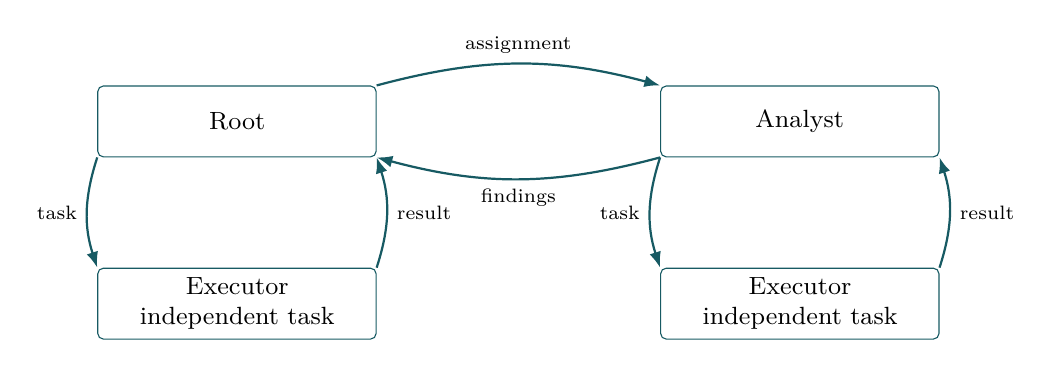
\begin{tikzpicture}[
  box/.style={draw=accent,rounded corners=2pt,align=center,font=\small,
    minimum height=9mm,text width=33mm},
  arrow/.style={-{Latex[length=2mm]},draw=accent,thick}]
\node[box] (root) {Root};
\node[box,right=36mm of root] (analyst) {Analyst};
\node[box,below=14mm of root] (rootexec) {Executor\\independent task};
\node[box,below=14mm of analyst] (analystexec) {Executor\\independent task};
\draw[arrow] (root.north east) to[bend left=15] node[above,font=\scriptsize]{assignment} (analyst.north west);
\draw[arrow] (analyst.south west) to[bend left=15] node[below,font=\scriptsize]{findings} (root.south east);
\draw[arrow] (root.south west) to[bend right=18] node[left,font=\scriptsize]{task} (rootexec.north west);
\draw[arrow] (rootexec.north east) to[bend right=18] node[right,font=\scriptsize]{result} (root.south east);
\draw[arrow] (analyst.south west) to[bend right=18] node[left,font=\scriptsize]{task} (analystexec.north west);
\draw[arrow] (analystexec.north east) to[bend right=18] node[right,font=\scriptsize]{result} (analyst.south east);
\end{tikzpicture}
\caption{Runtime delegation and return loops. Each executor assignment has its
own context and returns evidence to its requesting parent. This benchmark uses
the direct Root-to-executor route with local Root dispatch and low execution
effort.}
\label{fig:path}
\end{figure}

\section{Experimental protocol}

\subsection{Tasks and outcome definition}

SWE-bench evaluates issue resolution in real repositories through executable
tests~\cite{swebench}. We use every entry, in original order, from
\texttt{MariusHobbhahn/swe-bench-verified-mini}, a community-selected dataset
containing 50 tasks drawn from SWE-bench Verified~\cite{mini}. The fixed
manifest hash is published with the result summary. The scope of the reported
72\% HCCA resolution rate is these 50 selected tasks.

Each task starts from its specified base commit and issue text. Agent access
is restricted to the provided repository, issue and preinstalled dependencies.
The agent container has networking disabled. Host-side infrastructure relays
model requests, keeping model credentials outside the task container. Agents
receive no historical answers or patches. Official evaluation uses the generated
prediction against the SWE-bench task tests.

Let $r_i=1$ for an official resolved result and $r_i=0$ otherwise. An unfinished
task also receives $r_i=0$. The reported score is
\begin{equation}
  R = \frac{1}{50}\sum_{i=1}^{50} r_i.
\end{equation}
HCCA has 49 official reports and one unfinished task. Its official reports
contain 36 resolved and 13 unresolved outcomes. The unfinished task has no
official result and contributes zero credit. Its 17 model requests and all
associated token usage remain in the HCCA aggregate.

\subsection{Configurations and provenance}

The HCCA run uses a frozen v7 runtime and a run-local provider and scheduling
adapter. The source inventory contains 41 runtime files and 10 original
operations files, all checked against the frozen manifest. The adapter selects
GXWTF and the recorded model alias, uses two concurrent task slots and routes
requests through a dedicated relay. Each task has at most one outstanding model
request. Generation and evaluation share the two task slots.
The dedicated relay uses a process-local certificate-validation compatibility
setting for the gateway's expired certificate, recorded in the configuration.

The DSH comparator is the completed minimal-profile baseline~\cite{dsh}. It
is reused without additional baseline generation. Both arms use GXWTF and
\texttt{deepseek-v4.1-flash}, with two tasks concurrently. This is a sequential
comparison of two configurations run on separate dates. The public records
retain each arm's timing and source identities.

\begin{table}[ht]
\centering
\small
\begin{tabular}{p{57mm}p{45mm}p{43mm}}
\toprule
Setting & HCCA v7 (low) & DSH minimal high\\
\midrule
Provider and model alias & \multicolumn{2}{l}{GXWTF, \texttt{deepseek-v4.1-flash}}\\
Concurrent tasks & 2 & 2\\
Configured reasoning policy & Mixed by role & Single high-effort agent\\
Thinking/planning and analyst effort & high & \textemdash\\
Executor/reader effort & low & \textemdash\\
Observed benchmark request effort & 1,301 low, 0 high & baseline high\\
Initial model-planning stage & omitted & native minimal loop\\
Run date, UTC & November 12, 2026 & November 11, 2026\\
Active task time budget & 4,800 seconds & 4,800 seconds\\
Requested output token ceiling & omitted & omitted\\
Temperature and seed & omitted & server defaults\\
\bottomrule
\end{tabular}
\caption{Recorded experiment settings. The HCCA mixed role policy includes high
thinking/planning and analyst roles and low executor/reader roles. The direct
execution path produced 1,301 low requests and zero high requests. DSH uses
one high-effort agent. The context budget is a local estimate.}
\label{tab:config}
\end{table}

The HCCA soft executor context budget is 524,288 estimated tokens.
The executor starts directly, with no fixed planning-model call. Unlimited
executor rounds and shared calls remain subject to a 4,800-second active-runner
deadline. Preparation and official evaluation occur outside this budget. Both
arms omit client-specified model-output token caps. For this HCCA run, the
request adapter also omits temperature and seed.

\subsection{Accounting}

We reconcile HCCA runtime transport-attempt records with per-task request
exports and the dedicated relay, and obtain resolution from explicit official
report booleans. Each actual request belongs to the current frozen run,
including requests from failed or unfinished tasks. Earlier development runs
are outside these totals.

HCCA has \HRequests{} requests with complete usage. The baseline has
\BRequests{} actual requests, including 2,013 complete usage records and one
partial record. Baseline token aggregates below sum the complete records. The
unobserved usage of the partial record remains unknown. Exact baseline token
totals and cost therefore remain unknown.

We use common off-peak normalization at the experiment's archived rates, in
USD per million tokens, of 0.003 for cached input, 0.15 for uncached input and
0.60 for output~\cite{prices}. For counts $I_c$, $I_u$ and $O$, the normalized
cost is
\begin{equation}
  C = \frac{0.003 I_c + 0.15 I_u + 0.60 O}{10^6}.
\label{eq:cost}
\end{equation}
Provider-reported reasoning tokens are included in $O$ once. The normalized
cost is an accounting comparison at fixed prices. Actual GXWTF billing is a
separate quantity. Because the baseline has one partial record, we report its
known-complete cost as a lower bound.

\section{Results}

\begin{table}[ht]
\centering
\small
\begin{tabular}{lrr}
\toprule
Metric & HCCA v7 low & DSH minimal high\\
\midrule
Resolved / all tasks & 36 / 50 & 35 / 50\\
Officially evaluated & 49 & 50\\
Unfinished & 1 & 0\\
Actual model requests & \HRequests{} & \BRequests{}\\
Complete / partial usage records & 1,301 / 0 & 2,013 / 1\\
Input tokens & \HInput{} & \BInput{}\\
Cached input tokens & \HCached{} & \BCached{}\\
Uncached input tokens & \HMiss{} & \BMiss{}\\
Cached share of recorded input & \HCachePct{}\% & \BCachePct{}\%\\
Output tokens, including reasoning & \HOutput{} & \BOutput{}\\
Reasoning tokens within output & \HReasoning{} & \BReasoning{}\\
Other output tokens & \HOtherOutput{} & \BOtherOutput{}\\
Normalized cost, USD & \HCost{} & $\geq$\BCost{}\\
\bottomrule
\end{tabular}
\caption{Full-manifest outcomes and usage for HCCA v7 (low) and DSH minimal
high. DSH token counts and cache share
refer to its 2,013 complete records. Its remaining partial record is excluded
from these sums and retains unknown usage. All HCCA usage, including the
unfinished task, is included.}
\label{tab:results}
\end{table}

HCCA resolves 72\% of the fixed manifest and DSH resolves 70\%. The one-task
difference is small. The paired task outcomes are provided in the public
per-task accounting file. \PairedSentence{}

The HCCA phase runs from 11:58:43 to 12:58:53 UTC on November 12, 2026,
approximately 60 minutes 9.6 seconds including generation and evaluation.
The reused baseline's model-request window is 04:13:28 to 09:00:27 UTC on
November 11. Preparation, evaluation and host conditions affect elapsed time,
so these windows carry their recorded timing scope.

HCCA's \HCost{} USD normalized cost is at most 21.1\% of the baseline's
known-complete cost. This establishes at least a 78.9\% normalized-cost
reduction for the observed configurations, with baseline missing usage
increasing the baseline total if recovered. HCCA's normalized cost per resolved
task is \$\HCostPerResolved{}, while the baseline's known-complete cost per
resolved task is at least \$\BCostPerResolved{}.

Relative to the baseline's complete usage records, HCCA consumes approximately
65.4\% fewer input tokens and 83.8\% fewer output tokens. It makes 35.4\% fewer
actual requests. Both systems obtain substantial provider-reported cache reuse.
The cached share of recorded input is \HCachePct{}\% for HCCA and
\BCachePct{}\% for DSH.

\begin{figure}[ht]
\centering
\begin{minipage}[t]{.32\linewidth}\centering
\textbf{\scriptsize Input tokens (millions)}\\[2pt]
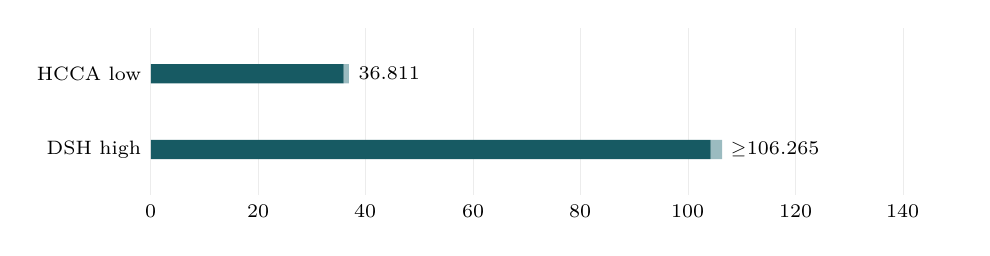
\begin{tikzpicture}\begin{axis}[
width=.98\linewidth,height=37mm,xbar stacked,bar width=7pt,
symbolic y coords={DSH high,HCCA low},ytick=data,
ymin={[normalized]-0.6},ymax={[normalized]1.6},xmin=0,xmax=150.89693332,
axis lines*=left,axis line style={draw=none},tick style={draw=none},
tick label style={font=\scriptsize},xmajorgrids,grid style={gray!15},enlarge y limits=false]
\addplot[fill=accent,draw=none] coordinates {(35.849984,{HCCA low}) (104.137856,{DSH high})};
\addplot[fill=cachelight,draw=none] coordinates {(0.960532,{HCCA low}) (2.12759,{DSH high})};
\node[anchor=west,font=\scriptsize] at (axis cs:36.810516,HCCA low){36.811};
\node[anchor=west,font=\scriptsize] at (axis cs:106.265446,DSH high){$\geq$106.265};
\end{axis}\end{tikzpicture}
{\scriptsize \textcolor{accent}{Cached}\quad \textcolor{cachelight}{Uncached}}
\end{minipage}
\hfill
\begin{minipage}[t]{.32\linewidth}\centering
\textbf{\scriptsize Output tokens (millions)}\\[2pt]
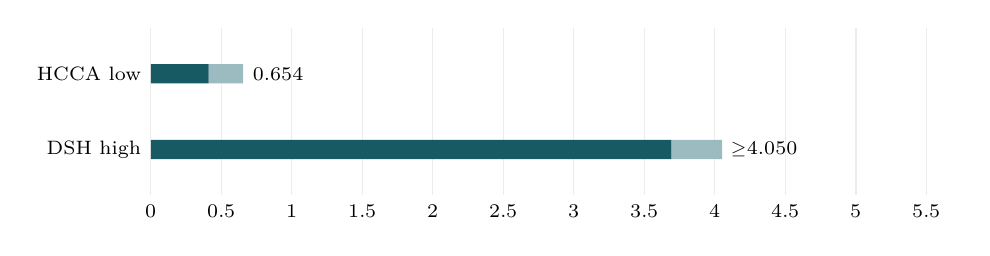
\begin{tikzpicture}\begin{axis}[
width=.98\linewidth,height=37mm,xbar stacked,bar width=7pt,
symbolic y coords={DSH high,HCCA low},ytick=data,
ymin={[normalized]-0.6},ymax={[normalized]1.6},xmin=0,xmax=5.752188539999999,
axis lines*=left,axis line style={draw=none},tick style={draw=none},
tick label style={font=\scriptsize},xmajorgrids,grid style={gray!15},enlarge y limits=false]
\addplot[fill=accent,draw=none] coordinates {(0.408903,{HCCA low}) (3.690753,{DSH high})};
\addplot[fill=cachelight,draw=none] coordinates {(0.245401,{HCCA low}) (0.360084,{DSH high})};
\node[anchor=west,font=\scriptsize] at (axis cs:0.654304,HCCA low){0.654};
\node[anchor=west,font=\scriptsize] at (axis cs:4.050837,DSH high){$\geq$4.050};
\end{axis}\end{tikzpicture}
{\scriptsize \textcolor{accent}{Reasoning}\quad \textcolor{cachelight}{Other output}}
\end{minipage}
\hfill
\begin{minipage}[t]{.32\linewidth}\centering
\textbf{\scriptsize Normalized cost (USD)}\\[2pt]
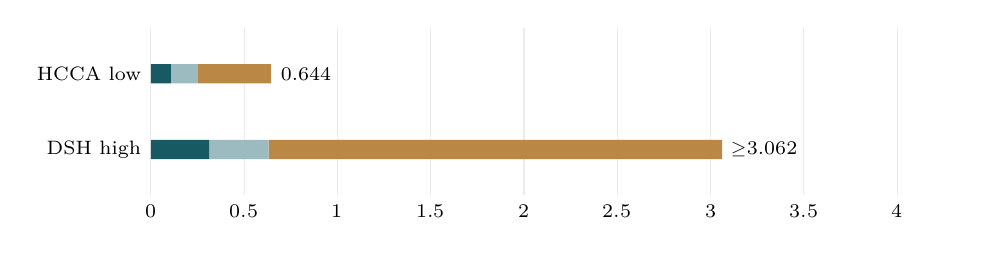
\begin{tikzpicture}\begin{axis}[
width=.98\linewidth,height=37mm,xbar stacked,bar width=7pt,
symbolic y coords={DSH high,HCCA low},ytick=data,
ymin={[normalized]-0.6},ymax={[normalized]1.6},xmin=0,xmax=4.34811706056,
axis lines*=left,axis line style={draw=none},tick style={draw=none},
tick label style={font=\scriptsize},xmajorgrids,grid style={gray!15},enlarge y limits=false]
\addplot[fill=accent,draw=none] coordinates {(0.107549952,{HCCA low}) (0.31241356800000003,{DSH high})};
\addplot[fill=cachelight,draw=none] coordinates {(0.14407979999999998,{HCCA low}) (0.3191385,{DSH high})};
\addplot[fill=outputgold,draw=none] coordinates {(0.39258239999999994,{HCCA low}) (2.4305022,{DSH high})};
\node[anchor=west,font=\scriptsize] at (axis cs:0.6442121519999999,HCCA low){0.644};
\node[anchor=west,font=\scriptsize] at (axis cs:3.062054268,DSH high){$\geq$3.062};
\end{axis}\end{tikzpicture}
{\scriptsize \textcolor{accent}{Cached input}\quad \textcolor{cachelight}{Uncached input}\quad \textcolor{outputgold}{Output}}
\end{minipage}

\caption{Input, output and normalized-cost composition for HCCA v7 (low)
and DSH minimal high. DSH bars show the
known-complete usage minimum. Reasoning is already part of output. Input
categories and output are priced separately using Equation~\ref{eq:cost}.}
\label{fig:usage}
\end{figure}

\section{Interpreting token consumption}

\subsection{Request count and input size}

Total input is the sum of prompt sizes over requests. Consequently, both the
number of requests and the average input per request affect token consumption.
Across its complete records, HCCA averages approximately 28,294 input tokens
per request. DSH's 2,013 complete records average approximately 52,790 input
tokens per request. These are request-weighted averages over repeated
conversation histories. They do not measure unique repository text or the
number of bytes a user supplied.

The observed input reduction combines fewer requests with smaller average
requests. Shared worker prefixes and local execution history provide a
mechanism for limiting what must enter a parent context. The direct-executor
route also avoids a fixed planning pass. This experiment changes several
properties together, so it does not identify a separate numerical contribution
for either mechanism.

\subsection{Cache reuse and monetary contribution}

Provider-reported cache counters quantify the portion of input charged at the
cached rate. Both arms have a high cached share, with the baseline's recorded
share higher than HCCA's. HCCA has lower cached and uncached input totals in
absolute terms. This combination explains how a configuration can consume less
input while having a slightly lower cache-hit fraction.

A shared prompt is an implementation property, whereas a provider cache hit
is an observation about serving behavior. Cache counters alone cannot reveal
the exact prefix that was reused or attribute hits to a particular instruction.
The source and configuration record establishes the intended stable-prefix
layout. The experiment establishes aggregate cache reuse reported by GXWTF.
Direct byte-level prefix and cache-placement measurements would be needed to
estimate a causal caching benefit.

At the normalization rates, HCCA's cost divides into approximately
\$0.107550 for cached input, \$0.144080 for uncached input and \$0.392582 for
output. Output therefore represents about 60.9\% of its normalized cost. The
same rates make output about 79.4\% of the baseline's known-complete cost.
The relative weights depend on the chosen common prices.

\subsection{Reasoning and other output}

HCCA's \HOutput{} output tokens include \HReasoning{} reasoning tokens.
The baseline's complete records contain \BOutput{} output tokens, including
\BReasoning{} reasoning tokens. The corresponding other-output counts are
\HOtherOutput{} and \BOtherOutput{}. We derive these counts by subtraction
from provider usage, and the category can include tool-call arguments as well
as visible text.

Approximately 96.6\% of the output-token difference between the recorded
aggregates is in the provider's reasoning field. Reasoning represents 62.5\%
of HCCA output and 91.1\% of baseline output. This arithmetic makes the
low-versus-high reasoning-effort difference a material interpretation issue.
Prompts, tools, number of turns and repair trajectories also differ. An
equal-effort ablation would be needed to estimate the portion caused by context
organization alone.

\section{Limitations and reproducibility}

\subsection{Scope of inference}

This is one run per configuration on a fixed community-selected 50-task
dataset. The tasks and their repository distribution can influence both
accuracy and cost. A one-task resolution advantage on this manifest offers
limited evidence about the ordering of the systems on other tasks. Paired
outcomes are reported to make the comparison inspectable. Repeated trials and
a larger independently specified task set would quantify variability.

Earlier runtime versions were iteratively developed and evaluated on this
same manifest. The present comparison is a development-benchmark measurement.

The configurations share an endpoint, model alias and task-concurrency setting.
They differ in reasoning effort, prompts, tool interfaces, history management
and execution policy, and were run on different dates. A model alias does not
establish identical underlying serving weights across dates. The baseline is
reused, so provider state and host conditions were not synchronized.

The current run exercises direct execution. It leaves reader isolation,
multi-level decomposition, multiple collaborating workers and interactive user
guidance without benchmark-specific efficacy estimates. HCCA Official 0.2.1
also includes packaging and Windows/DSH integration work beyond the frozen
snapshot. Those distribution features require their own evaluation.

The unfinished task receives zero score credit, and all observed usage is
included. Its
missing official result is retained as null in the public data, alongside a
zero score contribution. Baseline partial usage remains unknown. These choices
preserve the fixed denominator and observed expenditure.

\subsection{Published artifacts}

The repository publishes a versioned summary, one accounting row per task,
this paper and its XeLaTeX source~\cite{artifacts}. The records include task
identifiers, explicit outcomes, complete-usage counts, request totals,
normalized-cost components and provenance hashes. The source inventory hash
identifies the frozen runtime independently of subsequent distribution
releases. Historical v6 results retain their own filenames and configurations.

Raw task data, repository images, API credentials and full model traces are
maintained separately from the lightweight public distribution. Public hashes
provide provenance anchors. Re-execution additionally requires the exact task
data, prepared repositories, provider access and a matching runtime snapshot.
Preparation, generation, official evaluation and usage aggregation are distinct
steps in the recorded workflow.

The machine-readable summary links the verified source inventory and task
manifest to per-task results and run timestamps. Terminal accounting closes
the run as 49 evaluated tasks and one unfinished task.

\section{Conclusion}

On the fixed 50-task community Verified Mini manifest, frozen HCCA v7 with low
reasoning effort resolves 36 tasks at \$\HCost{} normalized cost, including one
unfinished task in the
denominator and all consumed usage. The reused DSH minimal high baseline
resolves 35 tasks with known-complete normalized cost of at least
\$\BCost{}. HCCA uses fewer requests, smaller average input requests and less
reported reasoning output in this comparison. Both configurations obtain high
provider-reported input-cache reuse.

\begin{thebibliography}{9}
\small
\raggedright
\bibitem{swebench}
Carlos E. Jimenez, John Yang, Alexander Wettig, Shunyu Yao, Kexin Pei,
Ofir Press and Karthik R. Narasimhan.
\emph{SWE-bench\textup{:} Can Language Models Resolve Real-World GitHub Issues?}
ICLR, 2024. \url{https://openreview.net/forum?id=VTF8yNQM66}.

\bibitem{mini}
Marius Hobbhahn. \emph{swe-bench-verified-mini}. Dataset repository.
\url{https://huggingface.co/datasets/MariusHobbhahn/swe-bench-verified-mini}.
Fixed task manifest and data hashes accompany this report.

\bibitem{dsh}
DeepSeek-AI. \emph{DeepSeek Harness}. 2026.
\url{https://github.com/deepseek-ai/deepseek-harness}.
The experiment reuses the project's recorded minimal high-effort baseline.

\bibitem{prices}
DeepSeek. \emph{Models and Pricing}.
\url{https://api-docs.deepseek.com/quick_start/pricing/}.
Common off-peak rates are frozen in the experiment's published accounting.

\bibitem{artifacts}
HCCA Project. \emph{Frozen-v7 Verified Mini results and accounting}.
November 12, 2026.
\url{https://github.com/klarisaka/HCCA-Official/blob/main/reports/verified50-hcca-v7-vs-dsh-2026-11-12-summary.json}.
Runtime distribution at \url{https://github.com/klarisaka/HCCA-Official}.
\end{thebibliography}

\end{document}
